\documentclass{beamer}

\usepackage{preamble}

\begin{document}

\begin{frame}
    \titlepage
\end{frame}

\begin{frame}{Outline}
    \tableofcontents
\end{frame}

\tikzset{g/.style={
            prefix after command= {\pgfextra{\tikzset{every label/.style={color=green,above left}}}}
}
}

\tikzset{r/.style={
            prefix after command= {\pgfextra{\tikzset{every label/.style={red,above left}}}}
}
}

\tikzset{o/.style={
            prefix after command= {\pgfextra{\tikzset{every label/.style={orange,above left}}}}
}
}

\section{Examples}

\subsection{blacklist}

\begin{example}
    Consider the following network where we want to check a blacklist
    property, i.e. no packets arrive at $d$:
    \begin{center}
        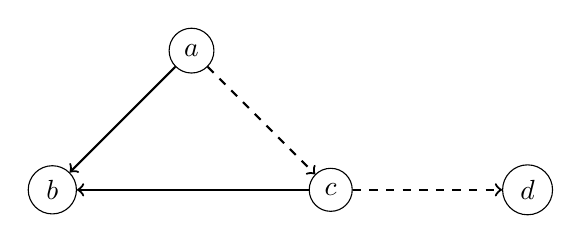
\begin{tikzpicture}[node distance={25mm},
                main/.style = {draw, circle},
                s/.style = {->,thick},
                d/.style = {->,thick,dashed} ]
            \node[main] (b) {$b$};
            \node[main] (a) [above right of=b] {$a$};
            \node[main] (c) [below right of=a] {$c$};
            \node[main] (d) [right of=c] {$d$};
            \draw[s] (a) -- (b);
            \draw[d] (a) -- (c);
            \draw[s] (c) -- (b);
            \draw[d] (c) -- (d);
        \end{tikzpicture}
    \end{center}
    We define this network using the following DyNetKAT term:
    \begin{align*}
        S_{xy}  & = sw = x \cdot sw \la y              \\
        P       & = u!S_{ac}                         \\
        Q       & = u!S_{cd}                         \\
        N_{x,y} & = (S_x+S_y)^* \oplus u?x';N_{x',y}
        \oplus u?y';N_{x,y'}                         \\
        SDN     & = \delta_{\mathcal{L}} (N_{ab,cb} 
        \parallel P \parallel Q)
    \end{align*}
    Where $\mathcal{L} = \s{u!S_{ac},u?S_{ac},u!S_{cd},u?S_{cd}}$.
    We may rewrite the terms as follows:
    \begin{align*}
        N_{ab,cb} & = (S_{ab} + S_{cb})^* \oplus u?S_{ac};N_{ac,cb}
        \oplus u?S_{cd};N_{ab,cd}                                   \\
        N_{ac,cb} & = (S_{ac}+S_{cb})^* \oplus u?S_{cd};N_{ac,cd}   \\
        N_{ab,cd} & = (S_{ab}+S_{cd})^* \oplus u?S_{ac};N_{ac,cd}   \\
        N_{ac,cd} & = (S_{ac}+S_{cd})^*
    \end{align*}
    We consider this network under the situation that a single packet 
    arrived at $a$.
    Thus we assume that a single packet $\sigma$ is arrived where 
    $\sigma(sw) = a$.
    Under this condition, we can replace the NetKAT terms with
    packet forwarding actions of the form $(\sigma, \sigma')$.
    We use $xy$ to denote an action of the form $(\sigma,\sigma')$
    where $\sigma(sw) = x$ and $\sigma(sw') = y$.
    For a DyNetKAT term $T$, we use $T^a$ to denote the term where 
    we have replaced all NetKAT policies with packet forwarding actions.
    Given a packet $\sigma$ where $\sigma(l) = a$ we can replace NetKAT
    Furthermore, we rename actions 
    $u?S_{ac},u!S_{ac},u?S_{cd},u!S_{cd}$ to $p,p',q,q'$, so we can 
    derive the following terms:
    \begin{align*}
        SDN^u & = \delta_{\mathcal{L}}( N'_{ab,cb} \parallel P \parallel Q) \\
        P & = p' \\
        Q & = q' \\
        N^u_{ab,cb} & = ab \oplus p;N^u_{ac,cb} \oplus q;N^u_{ab,cd} \\
        N^u_{ac,cb} & = ac \oplus ab \oplus q;N^u_{ac,cd}   \\
        N^u_{ab,cd} & = ab \oplus p;N^u_{ac,cd}             \\
        N^u_{ac,cd} & = ac \oplus ad 
    \end{align*}
    \begin{center}
        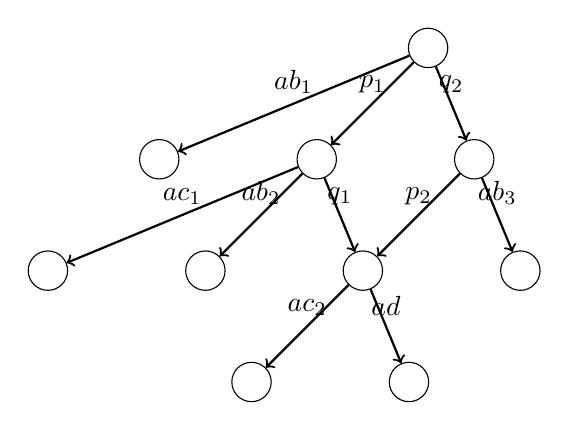
\begin{tikzpicture}[node distance={20mm},
                main/.style = {draw, circle,minimum width=5mm},
                s/.style = {->,thick}]
            \node[main] (s1) {};
            \node[main] (s3) [below left of=s1] {};
            \node[main] (s2) [left of=s3] {};
            \node[main] (s4) [right of=s3] {};
            \node[main] (s5) [below left of=s2] {};
            \node[main] (s6) [right of=s5] {};
            \node[main] (s7) [right of=s6] {};
            \node[main] (s8) [right of=s7] {};
            \node[main] (s9) [below left of=s7] {};
            \node[main] (s10) [right of=s9] {};
            \draw[s] (s1) -- node[above]{$ab_1$} (s2);
            \draw[s] (s1) -- node[above]{$p_1$}(s3);
            \draw[s] (s1) -- node[above]{$q_2$}(s4);
            \draw[s] (s3) -- node[above]{$ac_1$}(s5);
            \draw[s] (s3) -- node[above]{$ab_2$}(s6);
            \draw[s] (s3) -- node[above]{$q_1$}(s7);
            \draw[s] (s4) -- node[above]{$p_2$}(s7);
            \draw[s] (s4) -- node[above]{$ab_3$}(s8);
            \draw[s] (s7) -- node[above]{$ac_2$}(s9);
            \draw[s] (s7) -- node[above]{$ad$}(s10);
        \end{tikzpicture}
    \end{center}
    We may define the event structure $\mathrm{E} = (E,\#,\vdash,L,l)$ for $SDN'$ 
    where we have:
    \begin{align*}
        E = \s{ab_1,ab_2,ab_3,ac_1,ac_2,ad,p_1,p_2,q_1,q_2} \\
    \end{align*}
    Enabling relation the least one that satisfies:
    \begin{align*}
        & \e \vdash ab_1, \e \vdash p_1, \e \vdash q_2,
        \s{p_1} \vdash ac_1, \s{p_1} \vdash ab_2, \s{p_1} \vdash q_1,
        \s{q_1} \vdash p_2, \s{q_1} \vdash ab_3 \\
        & \s{p_1,q_1} \vdash ac_2, \s{p_1,q_1} \vdash ad,
        \s{p_2,q_2} \vdash ac_2, \s{p_2,q_2} \vdash ad
    \end{align*}
    And conflict relation the least one where:
    \begin{align*}
        \forall i,j,k. j \neq k \Rightarrow e_{i,k} \# e_{j,k} 
    \end{align*}
    Given an event structure $\mathrm{E} = (E,\#,\vdash)$, we define a safety
    property $\mathcal{P}$ as a subset of $\mathcal{F}(\mathrm{E})$.
    The safety property here is $d$ is being blacklist. 
    Thus, we define $ p \subseteq \mathcal{F}(\mathrm{E})$ to be the set of 
    configurations that do not contain an event of forwarding a packet to $d$.
    More formally we define $p$ as follows:
    \begin{align*}
        p = \s{s \subseteq E| \forall e \in s.  l(e) = (\sigma, \sigma')
         \Rightarrow \sigma'(l) \neq d }
    \end{align*}
    Finally, we can consider the set $\mathcal{P}(E) \setminus p$ as the 
    set of configurations for which we want to find the cause.
    Here, let $s = \mathcal{P}(E) \setminus p$.
    For our blacklist property $s$ contains all subsets of $E$ that contain $ad$.
    We wish to define nonexistence of a conflict between $p_1$ and $q_1$ 
    as a cause.
    We consider the witness $(C(p_2,q_2),\T,\T)$.
    If we set both $C(p_1,q_1)$ and $C(p_2,q_2)$ to true, then $ES$ for any 
    configuration $\sigma$ of $ES$ we have $\s{p_1,q_1} \not \in \sigma$ and
    $\s{p_1,q_2} \not \in \sigma$. Now, since $ad$ is only enabled either by
    $\s{p_1,q_1}$ or $\s{p_2,q_2}$, we can conclude that $ES$ can not have a
    configuration containing $ad$.
    For AC2(b), if we only set $C(p_2,q_2)$ to true, still ${p_1,q_1,ad}$ is 
    a configuration of $ES$ under any reset of other variables to their actual 
    values.
    Thus AC conditions are satisfied and we can declare $C(p_1,q_1)$ as a cause of
    the violation of the blacklist property.

\end{example}

\subsection{loop freedom}

\begin{frame}{Example: Loop Freedom}
    \begin{center}
        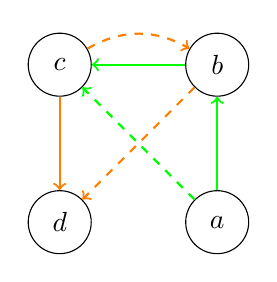
\begin{tikzpicture}[node distance={20mm},main/.style = {draw, circle,minimum size=8mm}]
            \node[main] (a)  {$a$};
            \node[main] (b) [above of=a]  {$b$};
            \node[main] (c) [left of=b] {$c$};
            \node[main] (d)  [below of=c] {$d$};
            \draw [->,green,thick] (a) -- (b);
            \draw [->,green,thick] (b) -- (c);
            \draw [->,orange,thick] (c) -- (d);
            \draw [->,green,thick,dashed] (a) -- (c);
            \draw [->,orange,thick,dashed] (c) edge[bend left] (b);
            \draw [->,orange,thick,dashed] (b) -- (d);
        \end{tikzpicture}
    \end{center}
    \begin{equation*}
        \begin{aligned}
            P           & = p!1                                               \\
            Q           & = q!1                                               \\
            S           & = F \oplus p?1;S_p \oplus q?1;S_q                   \\
            S_p         & = F_p \oplus q?1;F                                  \\
            S_q         & = F_q \oplus p?1;F                                  \\
            SDN         & = \delta_{\mathcal{L}}(SDN \parallel P \parallel Q) \\
            \mathcal{L} & = \s{p!1,p?1,q!1,q?1}
        \end{aligned}
        \qquad \qquad
        \begin{aligned}
            F    = & ab \oplus ac \oplus ad               \\
                   & \oplus bc \oplus bd \oplus cd        \\
            F_p  = & aac \oplus ad \oplus cd              \\
            F_q  = & ab \oplus ac \oplus ad               \\
                   & \oplus bc \oplus bb \oplus bd        \\
                   & \oplus        cb \oplus cc \oplus cd 
        \end{aligned}
    \end{equation*}
\end{frame}

\begin{frame}{Example: Loop Freedom}
    We can define $M(\s{p_2},q_2) = \F$ as a cause.

    Setting $M(\s{p_2},q_2)$ to true results in $EN(\e,q_2)$ become false
    neither $\s{q_2,bb}$ nor $\s{q_2,cc}$ are not configurations anymore
    We define:
    \begin{align*}
        \f{PV} & = \bigvee_{c \in C} c \in \mathcal{F}(ES) \\
        C      & = \s{c \subset E | \exists e \in c.
            l(e) = bb \vee l(e) = cc }
    \end{align*}
    \begin{center}
        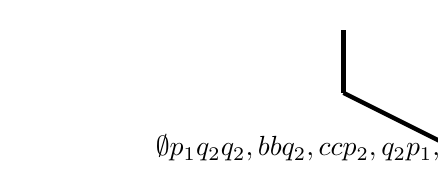
\begin{tikzpicture}[scale=0.8]
            \crd{0}{0}{$\emptyset$}
            \crd[below]{-2}{1}{$\s{p_1}$}
            \crd[below]{2}{1}{$\s{q_2}$}
            \crd[above]{2}{2}{$\s{q_2,bb}$}
            \crd[above]{4}{2}{$\s{q_2,cc}$}
            \crd[above]{0}{2}{$\s{p_2,q_2}$}
            \crd[left]{-2}{2}{$\s{p_1,q_1}$}
            \draw [ultra thick] (0,0) -- (2,1);
            \draw [ultra thick] (0,0) -- (-2,1);
            \draw [ultra thick] (2,1) -- (0,2);
            \draw [ultra thick] (2,1) -- (2,2);
            \draw [ultra thick] (2,1) -- (4,2);
            \draw [ultra thick] (-2,1) -- (-2,2);
        \end{tikzpicture}
    \end{center}
\end{frame}

\subsection{waypoint enforcement}

\begin{frame}
    \begin{center}
        \begin{tikzpicture}[node distance={20mm},main/.style = {draw, circle,minimum size=8mm}]
            \node[main] (h1)  {$h_1$};
            \node[main] (w) [right of=h1]  {$w$};
            \node[main] (s)  [above of=h1] {$s$};
            \node[main] (h2) [right of=s2]  {$h_2$};
            \draw[->] (h1) -- node[above]{1} (w);
            \draw[->] (w) --   (h2);
            \draw[->] (s) --  node[above]{3} (h2);
        \end{tikzpicture}
        \begin{tikzpicture}[node distance={20mm},main/.style = {draw, circle,minimum size=8mm}]
            \node[main] (h1)  {$h_1$};
            \node[main] (w) [right of=h1]  {$w$};
            \node[main] (s)  [above of=h1] {$s$};
            \node[main] (h2) [right of=s2]  {$h_2$};
            \draw[->] (h1) -- node[left]{2} (s);
            \draw[->] (s) --   node[above]{4}(w);
            \draw[->] (w) --   (h2);
        \end{tikzpicture}
    \end{center}
    Property:
    \begin{itemize}
        \item Property: waypoint enforcement
    \end{itemize}
    Current Behavior:
    \begin{enumerate}
        \item Replace path 1 with 2
    \end{enumerate}
\end{frame}

\begin{frame}
    \begin{center}
        \begin{tikzpicture}[node distance={20mm},main/.style = {draw, circle,minimum size=8mm}]
            \node[main] (h1)  {$h_1$};
            \node[main] (w) [right of=h1]  {$w$};
            \node[main] (s)  [above of=h1] {$s$};
            \node[main] (h2) [right of=s2]  {$h_2$};
            \draw[->] (h1) -- node[above]{1} (w);
            \draw[->,dashed] (h1) -- node[left]{2} (s);
            \draw[->] (w) --   (h2);
            \draw[->] (s) --  node[above]{3} (h2);
            \draw[->,dashed] (s) --  node[above]{4} (w);
        \end{tikzpicture}
        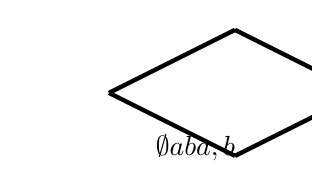
\begin{tikzpicture}[scale=0.8]
            \crd{0}{0}{$\emptyset$}
            \crd[left]{-2}{1}{$\s{a}$}
            \crd[right]{2}{1}{$\s{b}$}
            \crd[right]{0}{2}{$\s{a,b}$}
            \draw [ultra thick] (0,0) -- (2,1);
            \draw [ultra thick] (0,0) -- (-2,1);
            \draw [ultra thick] (-2,1) -- (0,2);
            \draw [ultra thick] (2,1) -- (0,2);
        \end{tikzpicture}
    \end{center}
    Events:
    \begin{itemize}
        \item $a$: Replace path 1 with 2
        \item $b$: Replace path 3 with 4
    \end{itemize}
    Counterexample: $\sigma = \s{a}$
\end{frame}


\subsection{invalid drop}
\begin{frame}
    \begin{center}
        \begin{tikzpicture}[node distance={20mm},main/.style = {draw, circle}]
            \node[main] (a)  {$a$};
            \node[main] (s) [right of=a]  {$s$};
            \node[main] (b) [right of=s] {$b$};
            \node[main] (c) [above of=s] {$c$};
            \draw (a) -- (s);
            \draw[dashed] (s) -- (c);
            \draw (s) -- (b);
        \end{tikzpicture}
    \end{center}
    Property:
    \begin{itemize}
        \item Property: allow packets from $b$ after a packet is sent toward it
    \end{itemize}
    Current Behavior:
    \begin{enumerate}
        \item $a$ sends a packet to $s$
        \item $s$ sends an event to $c$
        \item $b$ sends a packet to $s$
        \item $s$ drops the $b$'s packet
        \item $c$ sends a command to install a rule for allowing packets from $b$
    \end{enumerate}
\end{frame}

\begin{frame}
    \begin{center}
        \begin{tikzpicture}[node distance={20mm},main/.style = {draw, circle}]
            \node[main] (a)  {$a$};
            \node[main] (s) [right of=a]  {$s$};
            \node[main] (b) [right of=s] {$b$};
            \node[main] (c) [above of=s] {$c$};
            \draw (a) -- (s);
            \draw[dashed] (s) -- (c);
            \draw (s) -- (b);
        \end{tikzpicture}
        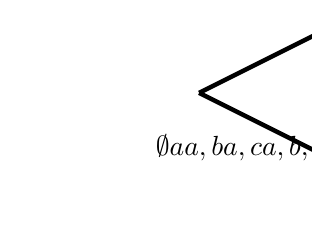
\begin{tikzpicture}[scale=0.8]
            \crd[left]{0}{-1}{$\emptyset$}
            \crd{0}{0}{$\s{a}$}
            \crd[left]{-2}{1}{$\s{a,b}$}
            \crd[right]{2}{1}{$\s{a,c}$}
            \crd[right]{0}{2}{$\s{a,b,c}$}
            \draw [ultra thick] (0,-1) -- (0,0);
            \draw [ultra thick] (0,0) -- (2,1);
            \draw [ultra thick] (0,0) -- (-2,1);
            \draw [ultra thick] (-2,1) -- (0,2);
            \draw [ultra thick] (2,1) -- (0,2);
        \end{tikzpicture}
    \end{center}
    Events:
    \begin{itemize}
        \item $a$: the arrival of a packet from $a$ at $s$ and sending event to $c$
        \item $b$: the arrival of a packet from $b$ at $s$
        \item $c$: the arrival of a command to allow packets from $b$
    \end{itemize}
    Enabling: $\e \vdash a, \s{a} \vdash b, \s{a} \vdash c$

    Counterexample: $\sigma = \s{a}$
\end{frame}


\subsection{congestion}
\begin{frame}
    \begin{center}
        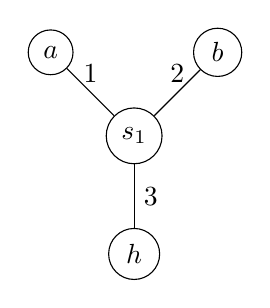
\begin{tikzpicture}[node distance={15mm},main/.style = {draw, circle}]
            \node[main] (s) {$s_1$};
            \node[main] (h) [below of=s] {$h$};
            \node[main] (a) [above left of=s]{$a$};
            \node[main] (b) [above right of=s]{$b$};
            \draw (a) --  node[above]{1}(s);
            \draw (b) --  node[above]{2}(s);
            \draw (s) --  node[right]{3}(h);
        \end{tikzpicture}
    \end{center}
    Property:
    \begin{itemize}
        \item at least two packets traversing link 3
    \end{itemize}
    Current Behavior:
    \begin{enumerate}
        \item forwarding a packet from 1 to 3
        \item forwarding a packet from 2 to 3
    \end{enumerate}
\end{frame}

\begin{frame}
    \begin{center}
        \begin{center}
            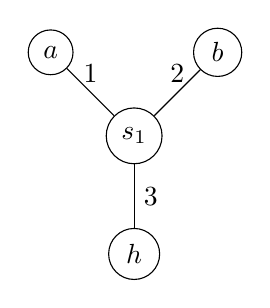
\begin{tikzpicture}[node distance={15mm},main/.style = {draw, circle}]
                \node[main] (s) {$s_1$};
                \node[main] (h) [below of=s] {$h$};
                \node[main] (a) [above left of=s]{$a$};
                \node[main] (b) [above right of=s]{$b$};
                \draw (a) --  node[above]{1}(s);
                \draw (b) --  node[above]{2}(s);
                \draw (s) --  node[right]{3}(h);
            \end{tikzpicture}
        \end{center}
        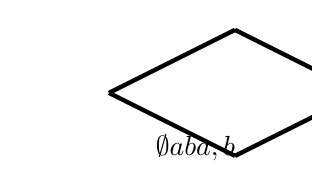
\begin{tikzpicture}[scale=0.8]
            \crd{0}{0}{$\emptyset$}
            \crd[left]{-2}{1}{$\s{a}$}
            \crd[right]{2}{1}{$\s{b}$}
            \crd[right]{0}{2}{$\s{a,b}$}
            \draw [ultra thick] (0,0) -- (2,1);
            \draw [ultra thick] (0,0) -- (-2,1);
            \draw [ultra thick] (-2,1) -- (0,2);
            \draw [ultra thick] (2,1) -- (0,2);
        \end{tikzpicture}
    \end{center}
    Events:
    \begin{itemize}
        \item $a$: Forwarding a packet from 1 to 3
        \item $b$: Forwarding a packet from 2 to 3
    \end{itemize}
    Counterexample: $\sigma = \s{a,b}$
\end{frame}

\begin{frame}
    \begin{center}
        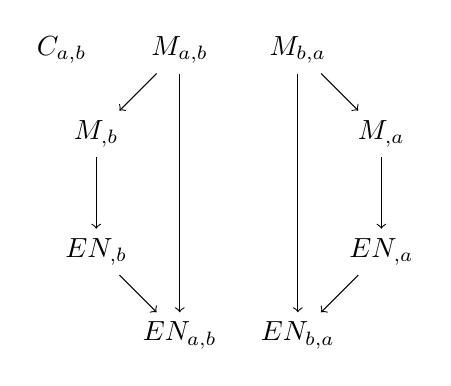
\begin{tikzpicture}[node distance=15mm]
            \node (mab) {$M_{\s{a},b}$};
            \node (mea) [below left of=mab] {$M_{\e,b}$};
            \node (eea) [below of=mea] {$EN_{\e,b}$};
            \node (eab) [below right of=eea]{$EN_{\s{a},b}$};
            \draw[->] (mab) -- (mea);
            \draw[->] (mea) -- (eea);
            \draw[->] (eea) -- (eab);
            \draw[->] (mab) -- (eab);

            \node (mba) [right of=mab] {$M_{\s{b},a}$};
            \node (meb) [below right of=mba] {$M_{\e,a}$};
            \node (eeb) [below of=meb] {$EN_{\e,a}$};
            \node (eba) [below left of=eeb]{$EN_{\s{b},a}$};
            \draw[->] (mba) -- (meb);
            \draw[->] (meb) -- (eeb);
            \draw[->] (eeb) -- (eba);
            \draw[->] (mba) -- (eba);

            \node (cab) [left of=mab] {$C_{a,b}$};

        \end{tikzpicture}
        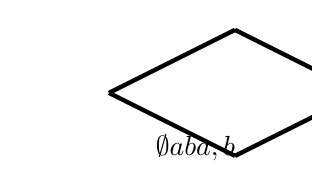
\begin{tikzpicture}[scale=0.8]
            \crd{0}{0}{$\emptyset$}
            \crd[left]{-2}{1}{$\s{a}$}
            \crd[right]{2}{1}{$\s{b}$}
            \crd[right]{0}{2}{$\s{a,b}$}
            \draw [ultra thick] (0,0) -- (2,1);
            \draw [ultra thick] (0,0) -- (-2,1);
            \draw [ultra thick] (-2,1) -- (0,2);
            \draw [ultra thick] (2,1) -- (0,2);
        \end{tikzpicture}
    \end{center}
    \begin{itemize}
        \item Counterexample: $\sigma = \s{a,b}$
        \item Cause: $C(a,b) = \F$
        \item Witness: $(\e,\e, \T)$
    \end{itemize}
\end{frame}

\begin{frame}
    \begin{center}
        \begin{tikzpicture}[node distance=15mm]
            \node[r,label=$\F$] (mab) {$M_{\s{a},b}$};
            \node[g,label=$\T$](mea) [below left of=mab] {$M_{\e,b}$};
            \node[g,label=$\T$](eea) [below of=mea] {$EN_{\e,b}$};
            \node[g,label=$\T$](eab) [below right of=eea]{$EN_{\s{a},b}$};
            \draw[->] (mab) -- (mea);
            \draw[->] (mea) -- (eea);
            \draw[->] (eea) -- (eab);
            \draw[->] (mab) -- (eab);

            \node [r,label=$\F$](mba) [right of=mab] {$M_{\s{b},a}$};
            \node [g,label=$\T$](meb) [below right of=mba] {$M_{\e,a}$};
            \node [g,label=$\T$](eeb) [below of=meb] {$EN_{\e,a}$};
            \node [g,label=$\T$](eba) [below left of=eeb]{$EN_{\s{b},a}$};
            \draw[->] (mba) -- (meb);
            \draw[->] (meb) -- (eeb);
            \draw[->] (eeb) -- (eba);
            \draw[->] (mba) -- (eba);

            \node [r,label=$\F$] (cab) [left of=mab] {$C_{a,b}$};

        \end{tikzpicture}
        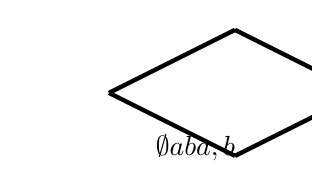
\begin{tikzpicture}[scale=0.8]
            \crd{0}{0}{$\emptyset$}
            \crd[left]{-2}{1}{$\s{a}$}
            \crd[right]{2}{1}{$\s{b}$}
            \crd[right]{0}{2}{$\s{a,b}$}
            \draw [ultra thick] (0,0) -- (2,1);
            \draw [ultra thick] (0,0) -- (-2,1);
            \draw [ultra thick] (-2,1) -- (0,2);
            \draw [ultra thick] (2,1) -- (0,2);
        \end{tikzpicture}
    \end{center}
\end{frame}


\begin{frame}
    \begin{center}
        \begin{tikzpicture}[node distance=15mm]
            \node [r,label=$\F$](mab) {$M_{\s{a},b}$};
            \node[g,label=$\T$](mea)     [below left of=mab] {$M_{\e,b}$};
            \node[g,label=$\T$](eea)    [below of=mea] {$EN_{\e,b}$};
            \node[g,label=$\T$](eab)    [below right of=eea]{$EN_{\s{a},b}$};
            \draw[->] (mab) -- (mea);
            \draw[->] (mea) -- (eea);
            \draw[->] (eea) -- (eab);
            \draw[->] (mab) -- (eab);

            \node [r,label=$\F$](mba) [right of=mab] {$M_{\s{b},a}$};
            \node [g,label=$\T$](meb) [below right of=mba] {$M_{\e,a}$};
            \node [g,label=$\T$](eeb) [below of=meb] {$EN_{\e,a}$};
            \node [g,label=$\T$](eba) [below left of=eeb]{$EN_{\s{b},a}$};
            \draw[->] (mba) -- (meb);
            \draw[->] (meb) -- (eeb);
            \draw[->] (eeb) -- (eba);
            \draw[->] (mba) -- (eba);

            \node [o,label=$\not \F \T$] (cab) [left of=mab] {$C_{a,b}$};

        \end{tikzpicture}
        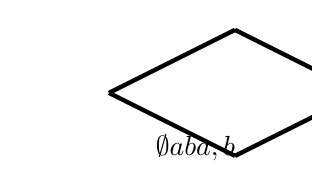
\begin{tikzpicture}[scale=0.8]
            \crd{0}{0}{$\emptyset$}
            \crd[left]{-2}{1}{$\s{a}$}
            \crd[right]{2}{1}{$\s{b}$}
            \crd[right]{0}{2}{$\s{a,b}$}
            \draw [ultra thick] (0,0) -- (2,1);
            \draw [ultra thick] (0,0) -- (-2,1);
            \draw [ultra thick] (-2,1) -- (0,2);
            \draw [ultra thick] (2,1) -- (0,2);
        \end{tikzpicture}
    \end{center}
\end{frame}

\begin{frame}
    \begin{center}
        \begin{tikzpicture}[node distance=15mm]
            \node[r,label=$\F$](mab) {$M_{\s{a},b}$};
            \node[g,label=$\T$](mea)     [below left of=mab] {$M_{\e,b}$};
            \node[g,label=$\T$](eea)    [below of=mea] {$EN_{\e,b}$};
            \node[g,label=$\T$](eab)    [below right of=eea]{$EN_{\s{a},b}$};
            \draw[->] (mab) -- (mea);
            \draw[->] (mea) -- (eea);
            \draw[->] (eea) -- (eab);
            \draw[->] (mab) -- (eab);

            \node [r,label=$\F$](mba) [right of=mab] {$M_{\s{b},a}$};
            \node [g,label=$\T$](meb) [below right of=mba] {$M_{\e,a}$};
            \node [g,label=$\T$](eeb) [below of=meb] {$EN_{\e,a}$};
            \node [g,label=$\T$](eba) [below left of=eeb]{$EN_{\s{b},a}$};
            \draw[->] (mba) -- (meb);
            \draw[->] (meb) -- (eeb);
            \draw[->] (eeb) -- (eba);
            \draw[->] (mba) -- (eba);

            \node [g,label=$\T$] (cab) [left of=mab] {$C_{a,b}$};

        \end{tikzpicture}
        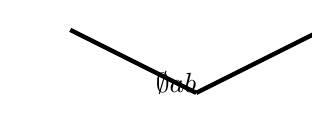
\begin{tikzpicture}[scale=0.8]
            \crd{0}{0}{$\emptyset$}
            \crd[left]{-2}{1}{$\s{a}$}
            \crd[right]{2}{1}{$\s{b}$}
            \draw [ultra thick] (0,0) -- (2,1);
            \draw [ultra thick] (0,0) -- (-2,1);
        \end{tikzpicture}
    \end{center}
\end{frame}


\end{document}